% D.27 扇形：半径 R=6，圆心角 120°
\documentclass[tikz,border=4pt]{standalone}
\usepackage{ctex}
\usepackage{amsmath}
\usetikzlibrary{calc}
\begin{document}
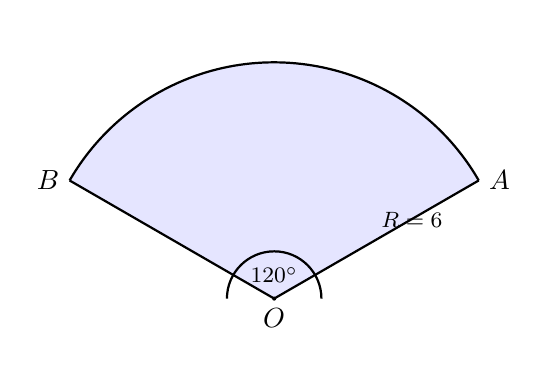
\begin{tikzpicture}[scale=0.5, thick]
  \coordinate (O) at (0, 0);
  \coordinate (A) at ({6*cos(30)},  {6*sin(30)});
  \coordinate (B) at ({6*cos(150)}, {6*sin(150)});

  \fill[blue!10] (O) -- (A) arc[start angle=30, end angle=150, radius=6] -- cycle;
  \draw (O) -- (A);
  \draw (O) -- (B);
  \draw (A) arc[start angle=30, end angle=150, radius=6];

  % 圆心角弧
  \draw (1.2, 0) arc[start angle=0, end angle=180, radius=1.2];
  \node at (0, 0.6) {\footnotesize $120^\circ$};

  \fill (O) circle (1.5pt);
  \node[below] at (O) {$O$};
  \node[right] at (A) {$A$};
  \node[left]  at (B) {$B$};
  \node at (3.5, 2) {\footnotesize $R=6$};
\end{tikzpicture}
\end{document}
